%%%%%%%%%%%%%%%%%%%%%%%%
% Microsoft Visual Studio
%%%%%%%%%%%%%%%%%%%%%%%%

\subsubsection{Purpose}
\noindent \ac{EMTG} depends on a compiler to generate an executable from the source code that will function on a user's machine. \ac{EMTG} is known to work with \hl{Microsoft Visual Studio 2022 Community Edition} and this will be utilized throughout this guide. Alternative compilers can be used for users skilled enough to adapt the instructions in this guide for their compiler of choice.

\subsubsection{Download Location}
\noindent The main page for the software distributions is in the following website: \\
\url{https://visualstudio.microsoft.com/vs/community/}

\noindent The software package needed for the EMTG version indicated in this guide can be obtained from the following location: \\
\emph{(In the event the url is no longer active, navigate to the aforementioned software website to find the specific version)} \\
\url{https://visualstudio.microsoft.com/thank-you-downloading-visual-studio/?sku=Community&channel=Release&version=VS2022&source=VSFeaturesPage&passive=true&tailored=cplus&cid=2031#cplusplus}. 

\noindent \hl{Executing the Visual Studio installer requires elevated privileges.}

\subsubsection{Dependency Installation Instructions}
\begin{enumerate}
	\item Execute the downloaded file and proceed through the install instructions utilizing the defaults unless otherwise indicated in the following steps
	\item Open Visual Studio once the installer completes
	\item Follow the prompts until you reach the ‘Get started’ prompt 
		\begin{figure}[H]
			\centering
			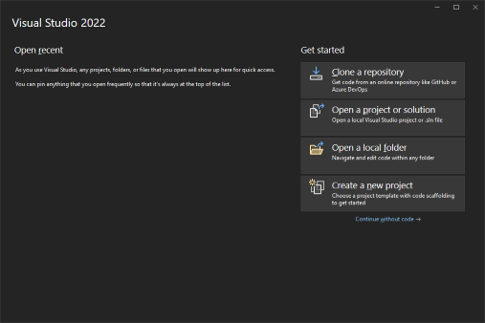
\includegraphics[width=0.9\linewidth]{../../../shared_latex_inputs/images/vstudio_init-menu.png}
			\caption{Visual Studios Startup Prompt}
		\end{figure}
	\item Click the “Continue without code” link
	\item Select ‘Tools’ -\textgreater  ‘Get Tools and Features ...’ in the tool menu
	\item Select the “Desktop development with C++” Workload
	\begin{enumerate}
		\item The selection of any other Workload and optional components is at the user's discretion
			\begin{figure}[H]
				\centering
				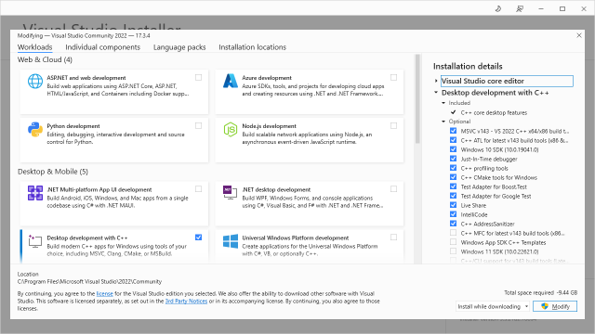
\includegraphics[width=0.95\linewidth]{../../../shared_latex_inputs/images/vstudio_cplusplus_menu.png}
				\caption{Visual Studios C++ Workload Selection}
			\end{figure}
	\end{enumerate}	
	\item Click the ‘Modify’ button, then continue through the prompts to complete the installation options needed for the remainder of the EMTG install steps
\end{enumerate}

